\documentclass[11pt,a4paper]{article}

\usepackage[margin=2.5cm]{geometry}
\usepackage[T1]{fontenc}
\usepackage[utf8]{inputenc}
\usepackage{lmodern}
\usepackage{microtype}
\usepackage{booktabs}
\usepackage{tabularx}
\usepackage{array}
\usepackage{graphicx}
\usepackage{xcolor}
\usepackage{listings}
\usepackage{caption}
\usepackage{subcaption}
\usepackage{hyperref}
\usepackage{amsmath}
\usepackage{parskip}
\usepackage{titlesec}
\usepackage{fancyhdr}
\usepackage{enumitem}
\usepackage{float}

% ── Colours ──────────────────────────────────────────────────────────────────
\definecolor{codeblue}{RGB}{0,90,160}
\definecolor{codegray}{RGB}{245,245,245}
\definecolor{codecomment}{RGB}{100,100,100}

% ── Code listings ─────────────────────────────────────────────────────────────
\lstset{
  language=Python,
  basicstyle=\ttfamily\small,
  keywordstyle=\color{codeblue}\bfseries,
  commentstyle=\color{codecomment}\itshape,
  stringstyle=\color{teal},
  backgroundcolor=\color{codegray},
  frame=single,
  rulecolor=\color{gray!40},
  framesep=4pt,
  xleftmargin=8pt,
  xrightmargin=4pt,
  breaklines=true,
  showstringspaces=false,
  numbers=none,
  captionpos=b
}

% ── Section formatting ────────────────────────────────────────────────────────
\titleformat{\section}{\large\bfseries}{}{0pt}{\thesection\quad}[\titlerule]
\titleformat{\subsection}{\normalsize\bfseries}{}{0pt}{\thesubsection\quad}

% ── Header / footer ───────────────────────────────────────────────────────────
\pagestyle{fancy}
\fancyhf{}
\rhead{\small NLP Final Project}
\lhead{\small Movie Review Sentiment Classifier}
\cfoot{\small\thepage}
\renewcommand{\headrulewidth}{0.4pt}

% ── Hyperref ──────────────────────────────────────────────────────────────────
\hypersetup{
  colorlinks=true,
  linkcolor=codeblue,
  urlcolor=codeblue,
  citecolor=codeblue,
  pdftitle={Movie Review Sentiment Classifier},
  pdfauthor={NLP Group}
}

% ─────────────────────────────────────────────────────────────────────────────
\begin{document}

% ── Title page ────────────────────────────────────────────────────────────────
\begin{titlepage}
  \centering
  \vspace*{2cm}

  {\Large\bfseries Natural Language Processing\par}
  \vspace{0.5cm}
  {\large Final Project Report\par}
  \vspace{2cm}

  {\Huge\bfseries Movie Review Sentiment\\[0.4em]Classification with NLTK\par}
  \vspace{2cm}

  {\large Juan Calle \quad Juan Francisco Gonz\'alez \quad Rodrigo Pelayo \quad Mar Blanco\par}
  \vspace{0.5cm}
  {\normalsize Academic Year 2025--2026\par}

  \vfill

  \begin{tabular}{ll}
    \textbf{Toolkit}   & NLTK 3.9.2 \\
    \textbf{Language}  & Python 3.9 \\
    \textbf{Dataset}   & \texttt{nltk.corpus.movie\_reviews} \\
    \textbf{Best acc.} & 76.50\% (Naive Bayes + BoW + POS) \\
  \end{tabular}

  \vspace{2cm}
  \today
\end{titlepage}

\tableofcontents
\newpage

% =============================================================================
\section{Introduction}
% =============================================================================

Sentiment analysis --- the automatic detection of opinion polarity in text --- is one of
the most widely studied tasks in Natural Language Processing. A working sentiment
classifier has immediate practical value: it can process thousands of reviews in seconds,
aggregate audience reaction to a film, and surface signals that would take human readers
hours to distil.

This project implements a \textbf{binary sentiment classifier} for movie reviews:
given a review text, the system predicts whether it expresses a \emph{positive} or
\emph{negative} opinion. The entire pipeline --- corpus access, text normalisation,
feature engineering, supervised learning, and evaluation --- is built with the
\textbf{Natural Language Toolkit (NLTK)}, the library studied throughout the course.

The main objectives are:
\begin{itemize}[noitemsep]
  \item Build a functional, reproducible sentiment classification pipeline.
  \item Demonstrate direct use of NLTK components covered in class (Chapters 2, 3, 5 and 6).
  \item Provide a clear justification for every design choice.
  \item Compare two classification algorithms and two feature schemes.
\end{itemize}

% =============================================================================
\section{Dataset}
% =============================================================================

We use \texttt{nltk.corpus.movie\_reviews}, a corpus shipped directly with NLTK. It
contains 2\,000 pre-tokenised movie reviews collected from the Internet Movie Database
(IMDb) and labelled by Pang and Lee~\cite{pang2002thumbs}. The class distribution is
perfectly balanced (Table~\ref{tab:dataset}).

\begin{table}[H]
  \centering
  \caption{Dataset statistics.}
  \label{tab:dataset}
  \begin{tabular}{lc}
    \toprule
    \textbf{Property} & \textbf{Value} \\
    \midrule
    Total reviews      & 2\,000 \\
    Positive reviews   & 1\,000 \\
    Negative reviews   & 1\,000 \\
    Class balance      & 50\% / 50\% \\
    Format             & Pre-tokenised word lists \\
    Train split (80\%) & 1\,600 documents \\
    Test split  (20\%) & 400 documents \\
    \bottomrule
  \end{tabular}
\end{table}

The corpus is accessed via the standard NLTK corpus API (Chapter~2):

\begin{lstlisting}[caption={Corpus access using the NLTK corpus API.}]
from nltk.corpus import movie_reviews

documents = [
    (list(movie_reviews.words(fileid)), category)
    for category in movie_reviews.categories()   # 'pos' or 'neg'
    for fileid in movie_reviews.fileids(category)
]
\end{lstlisting}

Documents were shuffled with a fixed random seed (\texttt{seed=42}) and split 80/20
into training and test sets, yielding \textbf{1\,600 training} and \textbf{400 test}
samples.

% =============================================================================
\section{Methodology}
% =============================================================================

\subsection{System Architecture}

Figure~\ref{fig:pipeline} summarises the end-to-end pipeline.

\begin{figure}[H]
  \centering
  \setlength{\fboxsep}{8pt}
  \fbox{%
    \begin{minipage}{0.86\textwidth}
      \centering
      \textbf{Raw corpus} (\texttt{movie\_reviews})\\[4pt]
      $\downarrow$ \textit{Ch02 --- corpus API}\\[4pt]
      \textbf{Preprocessing}:
      lowercase $\to$ remove stopwords $\to$ filter non-alpha $\to$ PorterStemmer\\[4pt]
      $\downarrow$ \textit{Ch02--03}\\[4pt]
      \textbf{Vocabulary selection}: \texttt{FreqDist} $\to$ top 2\,000 words\\[4pt]
      $\downarrow$ \textit{Ch02}\\[4pt]
      \textbf{Feature extraction}\\
      Exp.\,1: Boolean BoW $\quad|\quad$ Exp.\,2: Boolean BoW + POS adjective features\\[4pt]
      $\downarrow$ \textit{Ch05--06}\\[4pt]
      \textbf{Classification}: \texttt{NaiveBayesClassifier} / \texttt{DecisionTreeClassifier}\\[4pt]
      $\downarrow$ \textit{Ch06}\\[4pt]
      \textbf{Evaluation}: Accuracy, Precision, Recall, F1, Confusion Matrix
    \end{minipage}%
  }
  \caption{End-to-end sentiment classification pipeline.}
  \label{fig:pipeline}
\end{figure}

\subsection{NLTK Components and Justification}

This subsection describes every NLTK component used in the project, the chapter in
which it was introduced, and the reason it was chosen.

\subsubsection{Corpus Access --- \texttt{movie\_reviews} (Chapter~2)}

NLTK's corpus infrastructure provides a uniform interface: \texttt{.categories()},
\texttt{.fileids(category)}, and \texttt{.words(fileid)}. Using the built-in corpus
avoids external dependencies, is directly linked to the class material, and guarantees
a reproducible, labelled benchmark.

\subsubsection{Frequency Distribution --- \texttt{FreqDist} (Chapter~2)}

\texttt{FreqDist} computes word frequencies across all documents and selects the
\textbf{2\,000 most frequent stemmed tokens} as the feature vocabulary.

\begin{lstlisting}[caption={Vocabulary selection via \texttt{FreqDist}.}]
from nltk import FreqDist

all_words = FreqDist(word
    for (word_list, _) in documents
    for word in preprocess(word_list))
vocabulary = [w for (w, _) in all_words.most_common(2000)]
\end{lstlisting}

Using all ~40\,000 unique tokens as features would produce an extremely sparse and
noisy feature space. Restricting to the top-$N$ by frequency is the standard approach
shown in Chapter~6. Rare words carry insufficient statistical evidence to support
classification.

\subsubsection{Stopword Removal --- \texttt{stopwords} (Chapter~2)}

The English stopword list (179 function words: \emph{the}, \emph{is}, \emph{at},
\ldots) is removed during preprocessing. Stopwords carry no sentiment signal and would
displace informative tokens from the fixed-size vocabulary.

\subsubsection{Text Normalisation --- Tokenisation and Lowercasing (Chapter~3)}

Chapter~3 covers the normalisation pipeline. We apply \texttt{.lower()} and
\texttt{.isalpha()} filtering to remove punctuation tokens and case variants
(\emph{Film} vs.\ \emph{film}).

\subsubsection{Stemming --- \texttt{PorterStemmer} (Chapter~3)}

The Porter Stemmer reduces inflected forms to a common root:
\emph{running} $\to$ \texttt{run}, \emph{outstanding} $\to$ \texttt{outstand},
\emph{poorly} $\to$ \texttt{poorli}.

\begin{lstlisting}[caption={Preprocessing pipeline using \texttt{PorterStemmer}.}]
from nltk.stem import PorterStemmer
from nltk.corpus import stopwords

stop_words = set(stopwords.words("english"))
stemmer    = PorterStemmer()

def preprocess(word_list):
    return [stemmer.stem(w.lower())
            for w in word_list
            if w.isalpha() and w.lower() not in stop_words]
\end{lstlisting}

Stemming reduces vocabulary size and groups semantically related forms under a single
feature: reviews containing \emph{wasted} and \emph{waste} both activate
\texttt{contains(wast)}. The Porter algorithm was preferred over Lancaster (too
aggressive) and \texttt{WordNetLemmatizer} (requires POS context at every call) for its
balance between normalisation strength and computational cost.

\subsubsection{POS Tagging --- \texttt{pos\_tag} (Chapter~5)}

To test the hypothesis that opinion-bearing adjectives are a strong sentiment signal, we
extract adjectives (Penn Treebank tags: \texttt{JJ}, \texttt{JJR}, \texttt{JJS}) and
add two numeric features per document:

\begin{lstlisting}[caption={POS-augmented feature extraction.}]
from nltk import pos_tag

tagged = pos_tag(word_list[:200])
adjectives = {w.lower() for (w, tag) in tagged if tag.startswith("JJ")}
features["has_adjectives"] = bool(adjectives)
features["adj_count"]      = len(adjectives)
\end{lstlisting}

Adjectives are the primary lexical carriers of evaluation (\emph{excellent},
\emph{dull}, \emph{brilliant}, \emph{awful}). The \texttt{adj\_count} feature appeared
in the top-20 most informative features of Experiment~2 (ratio 4.4:1 toward positive),
confirming the linguistic hypothesis.

\subsubsection{Naive Bayes Classifier --- \texttt{NaiveBayesClassifier} (Chapter~6)}

The Naive Bayes classifier is the primary model, following the classification framework
from Chapter~6. It estimates the posterior probability of each class given the feature
vector under a conditional-independence assumption:

\[
  P(\text{class} \mid \mathbf{f}) \propto P(\text{class})
  \prod_{i} P(f_i \mid \text{class})
\]

\textbf{Justification:} Naive Bayes is well-suited to bag-of-words features because
(i)~it handles high-dimensional sparse spaces efficiently; (ii)~the independence
assumption is reasonable for unordered binary word-presence features; and (iii)~it is
the classifier demonstrated in Chapter~6 for exactly this type of task.

\subsubsection{Decision Tree Classifier --- \texttt{DecisionTreeClassifier} (Chapter~6)}

A decision tree classifier was trained for comparison. It recursively selects the most
informative feature at each node using information gain (entropy). The tree is trained
with \texttt{entropy\_cutoff=0.05}, \texttt{depth\_cutoff=100}, and
\texttt{support\_cutoff=10} to limit overfitting.

\subsubsection{Evaluation --- \texttt{accuracy} and \texttt{ConfusionMatrix} (Chapter~6)}

\begin{lstlisting}[caption={Evaluation using NLTK's built-in tools.}]
from nltk.classify import accuracy
from nltk         import ConfusionMatrix

acc = accuracy(classifier, test_set)

gold      = [cat for (_, cat) in test_set]
predicted = [classifier.classify(feat) for (feat, _) in test_set]
cm = ConfusionMatrix(gold, predicted)
print(cm.pretty_format(sort_by_count=True, show_percents=True))
\end{lstlisting}

In addition to accuracy, we compute per-class Precision, Recall, and F1-score to
account for any class-level asymmetries.

% =============================================================================
\section{Experiments and Results}
% =============================================================================

\subsection{Experiment 1 --- Bag-of-Words Features}

Each document is represented as a dictionary of Boolean features
\texttt{\{contains(w): True/False\}} over the 2\,000-word vocabulary.

\begin{table}[H]
  \centering
  \caption{Experiment 1 results --- BoW features.}
  \label{tab:exp1}
  \begin{tabular}{lc}
    \toprule
    \textbf{Classifier} & \textbf{Accuracy} \\
    \midrule
    Naive Bayes   & 76.00\% \\
    Decision Tree & 64.25\% \\
    \bottomrule
  \end{tabular}
\end{table}

\begin{table}[H]
  \centering
  \caption{Confusion matrix --- Naive Bayes, BoW (400 test samples).}
  \label{tab:cm1}
  \begin{tabular}{lccc}
    \toprule
    & \textbf{Predicted POS} & \textbf{Predicted NEG} & \textbf{Total} \\
    \midrule
    \textbf{Actual POS} & 135 (33.8\%) & 67 (16.8\%) & 202 \\
    \textbf{Actual NEG} &  29 \ (7.2\%)& 169 (42.2\%)& 198 \\
    \bottomrule
  \end{tabular}
\end{table}

\begin{table}[H]
  \centering
  \caption{Per-class metrics --- Naive Bayes, BoW.}
  \label{tab:metrics1}
  \begin{tabular}{lccc}
    \toprule
    \textbf{Class} & \textbf{Precision} & \textbf{Recall} & \textbf{F1} \\
    \midrule
    Positive & 0.8232 & 0.6683 & 0.7377 \\
    Negative & 0.7161 & 0.8535 & 0.7788 \\
    \bottomrule
  \end{tabular}
\end{table}

Table~\ref{tab:features} shows the top-20 most informative features learned by Naive
Bayes. Features are ranked by the likelihood ratio between the two classes.

\begin{table}[H]
  \centering
  \caption{Top-20 most informative features (Naive Bayes, BoW).}
  \label{tab:features}
  \small
  \begin{tabular}{llr}
    \toprule
    \textbf{Feature} & \textbf{Direction} & \textbf{Ratio} \\
    \midrule
    \texttt{contains(seagal)}     & negative & 9.6:1 \\
    \texttt{contains(outstand)}   & positive & 8.5:1 \\
    \texttt{contains(idiot)}      & negative & 7.1:1 \\
    \texttt{contains(mulan)}      & positive & 6.4:1 \\
    \texttt{contains(lame)}       & negative & 5.8:1 \\
    \texttt{contains(flynt)}      & positive & 5.7:1 \\
    \texttt{contains(damon)}      & positive & 5.5:1 \\
    \texttt{contains(stupid)}     & negative & 5.3:1 \\
    \texttt{contains(balanc)}     & positive & 5.2:1 \\
    \texttt{contains(poorli)}     & negative & 5.1:1 \\
    \texttt{contains(worst)}      & negative & 5.1:1 \\
    \texttt{contains(unfunni)}    & negative & 5.0:1 \\
    \texttt{contains(wast)}       & negative & 4.5:1 \\
    \texttt{contains(pointless)}  & negative & 4.4:1 \\
    \texttt{contains(laughabl)}   & negative & 4.4:1 \\
    \texttt{contains(uninterest)} & negative & 4.3:1 \\
    \texttt{contains(subtl)}      & positive & 4.1:1 \\
    \texttt{contains(era)}        & positive & 4.1:1 \\
    \texttt{contains(badli)}      & negative & 4.0:1 \\
    \texttt{contains(dull)}       & negative & 4.0:1 \\
    \bottomrule
  \end{tabular}
\end{table}

\subsection{Experiment 2 --- BoW + POS Adjective Features}

Experiment~2 extends Experiment~1 by adding \texttt{has\_adjectives} (Boolean) and
\texttt{adj\_count} (integer) features derived from \texttt{pos\_tag}.

\begin{table}[H]
  \centering
  \caption{Experiment 2 results --- BoW + POS features.}
  \label{tab:exp2}
  \begin{tabular}{lc}
    \toprule
    \textbf{Classifier} & \textbf{Accuracy} \\
    \midrule
    Naive Bayes   & 76.50\% \\
    Decision Tree & 62.75\% \\
    \bottomrule
  \end{tabular}
\end{table}

The \texttt{adj\_count} feature entered the top-20 most informative features at position
16 (ratio 4.4:1 toward positive), confirming that adjective density is a useful
signal for positive sentiment.

\subsection{Summary}

\begin{table}[H]
  \centering
  \caption{Overall results across all models and feature sets.}
  \label{tab:summary}
  \begin{tabular}{llc}
    \toprule
    \textbf{Classifier} & \textbf{Features} & \textbf{Accuracy} \\
    \midrule
    Naive Bayes   & BoW            & 76.00\% \\
    Decision Tree & BoW            & 64.25\% \\
    Naive Bayes   & BoW + POS      & \textbf{76.50\%} \\
    Decision Tree & BoW + POS      & 62.75\% \\
    \bottomrule
  \end{tabular}
\end{table}

\subsection{Word Frequency Analysis}

Figure~\ref{fig:freq} shows the 30 most frequent words after preprocessing. Function
words have been removed by the stopword filter, exposing content words such as
\emph{film}, \emph{movi}, \emph{stori}, and \emph{charact}. Figure~\ref{fig:catfreq}
contrasts word frequencies between positive and negative reviews.

\begin{figure}[H]
  \centering
  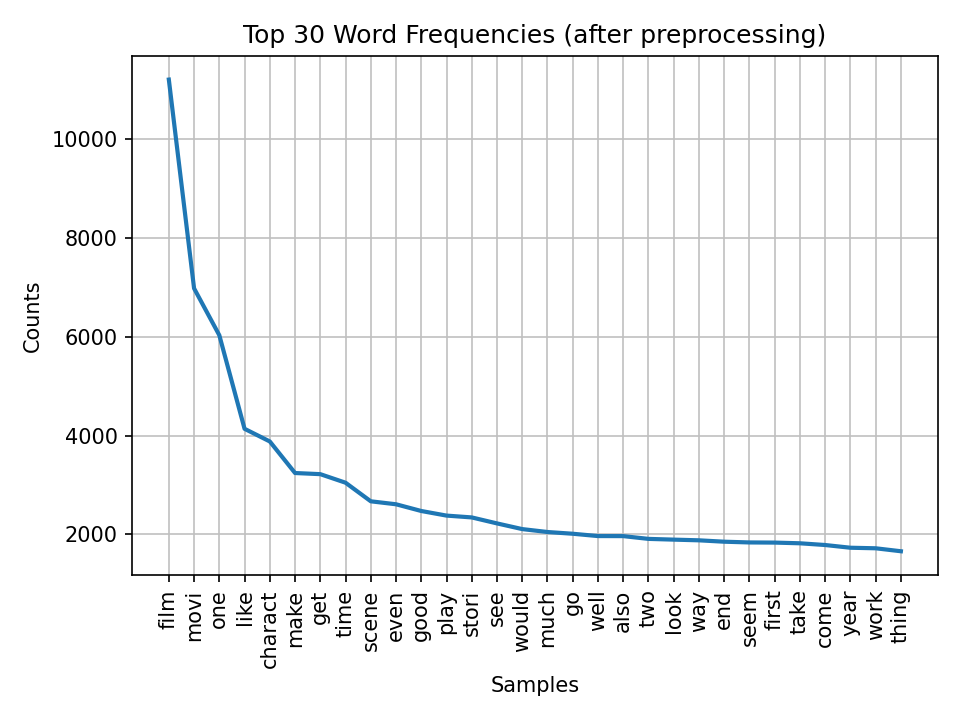
\includegraphics[width=0.85\textwidth]{frequency_distribution.png}
  \caption{Top-30 word frequencies across the full corpus (after preprocessing).}
  \label{fig:freq}
\end{figure}

\begin{figure}[H]
  \centering
  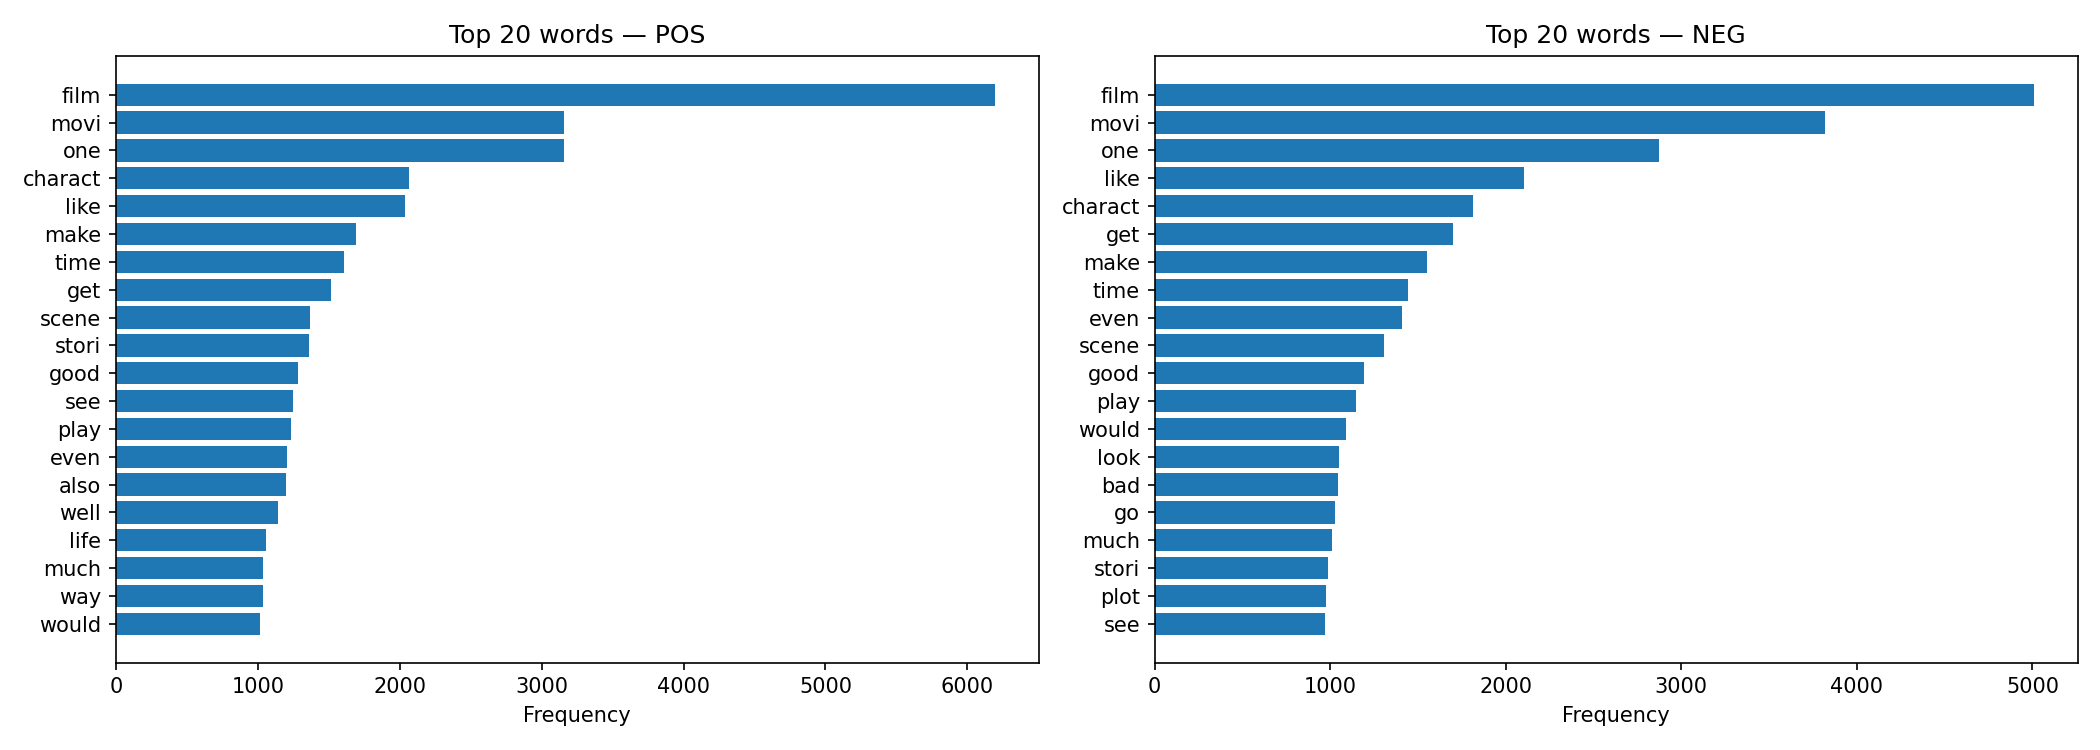
\includegraphics[width=\textwidth]{category_frequencies.png}
  \caption{Top-20 words per sentiment category. Positive reviews use more evaluative
           adjectives; negative reviews feature words expressing frustration and failure.}
  \label{fig:catfreq}
\end{figure}

% =============================================================================
\section{Discussion}
% =============================================================================

\subsection{Why Naive Bayes Outperforms Decision Tree}

Naive Bayes is well-calibrated for high-dimensional sparse binary features. A
2\,000-dimensional Boolean feature space is exactly the regime where it excels: each
feature probability is estimated independently, and the sparse structure does not
penalise the model. The decision tree must find axis-aligned splits in the same space
and tends to overfit individual review-specific tokens. The 12-percentage-point
accuracy gap (76\% vs.\ 64\%) confirms that Naive Bayes is the appropriate choice for
bag-of-words text classification.

\subsection{Why POS Features Help Marginally}

Adding \texttt{adj\_count} improved Naive Bayes by 0.5 percentage points. The effect is
small because the BoW features already capture most sentiment-bearing adjectives
individually (\texttt{contains(outstand)}, \texttt{contains(lame)}, etc.). The
\texttt{adj\_count} feature adds an orthogonal signal --- how opinion-rich is the
language overall? --- but its marginal contribution is limited given the already strong
lexical baseline.

\subsection{Most Informative Features --- Observations}

The top features fall into three groups:
\begin{enumerate}[noitemsep]
  \item \textbf{Stemmed sentiment adjectives and adverbs:} \texttt{outstand},
        \texttt{lame}, \texttt{worst}, \texttt{dull}, \texttt{poorli}, \texttt{unfunni}.
        These directly encode evaluative language.
  \item \textbf{Actor and film names:} \texttt{seagal} (Steven Seagal, associated with
        low-quality action films), \texttt{damon} (Matt Damon, associated with prestige
        films), \texttt{mulan} (Mulan, well-reviewed animated film), \texttt{flynt}
        (\emph{The People vs.\ Larry Flynt}, positively reviewed drama). The classifier
        learns domain-specific associations, not just generic sentiment words.
  \item \textbf{Evaluative nouns and verbs:} \texttt{wast}, \texttt{balanc},
        \texttt{subtl}. These carry implicit sentiment through their connotations.
\end{enumerate}

\subsection{Limitations}

\begin{itemize}[noitemsep]
  \item \textbf{No bigrams.} Phrase-level negation (\emph{not good}) is invisible to
        unigram BoW.
  \item \textbf{Fixed vocabulary size.} Rare but highly diagnostic terms are excluded.
  \item \textbf{Single train/test split.} Cross-validation would yield more stable
        accuracy estimates.
  \item \textbf{Partial POS tagging.} For efficiency, only the first 200 tokens of each
        review are tagged; full-document tagging would be more accurate.
\end{itemize}

% =============================================================================
\section{Conclusion}
% =============================================================================

This project has demonstrated a complete NLP pipeline for binary sentiment
classification of movie reviews, implemented exclusively with NLTK. The pipeline spans
corpus access (\texttt{movie\_reviews}, Chapter~2), text normalisation
(\texttt{PorterStemmer}, \texttt{stopwords}, Chapter~3), vocabulary selection
(\texttt{FreqDist}, Chapter~2), POS-augmented feature extraction (\texttt{pos\_tag},
Chapter~5), supervised classification (\texttt{NaiveBayesClassifier},
\texttt{DecisionTreeClassifier}, Chapter~6), and evaluation (\texttt{accuracy},
\texttt{ConfusionMatrix}, Chapter~6).

The best model --- Naive Bayes with Boolean BoW features augmented by adjective count
--- achieves \textbf{76.50\% accuracy} on a balanced 400-sample test set. Naive Bayes
outperforms Decision Trees by a large margin, consistent with the well-known suitability
of generative classifiers for sparse text features. The most informative features reveal
that the model learns genuine linguistic patterns: evaluative adjectives, domain-specific
actor associations, and sentiment adverbs all contribute to classification.

All code is available in \texttt{main.py} and can be executed with a single command
after installing \texttt{nltk} and \texttt{matplotlib}.

% =============================================================================
% References
% =============================================================================
\begin{thebibliography}{9}

\bibitem{pang2002thumbs}
  B.~Pang and L.~Lee,
  \emph{Thumbs up? Sentiment Classification using Machine Learning Techniques},
  in \textit{Proceedings of EMNLP 2002}, pp.~79--86, 2002.

\bibitem{nltkbook}
  S.~Bird, E.~Klein, and E.~Loper,
  \emph{Natural Language Processing with Python},
  O'Reilly Media, 2009.
  Available at \url{https://www.nltk.org/book/}.

\bibitem{porter1980}
  M.~F.~Porter,
  \emph{An Algorithm for Suffix Stripping},
  \textit{Program}, vol.~14, no.~3, pp.~130--137, 1980.

\end{thebibliography}

\end{document}
